\documentclass[1p]{elsarticle_modified}
%\bibliographystyle{elsarticle-num}

%\usepackage[colorlinks]{hyperref}
%\usepackage{abbrmath_seonhwa} %\Abb, \Ascr, \Acal ,\Abf, \Afrak
\usepackage{amsfonts}
\usepackage{amssymb}
\usepackage{amsmath}
\usepackage{amsthm}
\usepackage{scalefnt}
\usepackage{amsbsy}
\usepackage{kotex}
\usepackage{caption}
\usepackage{subfig}
\usepackage{color}
\usepackage{graphicx}
\usepackage{xcolor} %% white, black, red, green, blue, cyan, magenta, yellow
\usepackage{float}
\usepackage{setspace}
\usepackage{hyperref}

\usepackage{tikz}
\usetikzlibrary{arrows}

\usepackage{multirow}
\usepackage{array} % fixed length table
\usepackage{hhline}

%%%%%%%%%%%%%%%%%%%%%
\makeatletter
\renewcommand*\env@matrix[1][\arraystretch]{%
	\edef\arraystretch{#1}%
	\hskip -\arraycolsep
	\let\@ifnextchar\new@ifnextchar
	\array{*\c@MaxMatrixCols c}}
\makeatother %https://tex.stackexchange.com/questions/14071/how-can-i-increase-the-line-spacing-in-a-matrix
%%%%%%%%%%%%%%%

\usepackage[normalem]{ulem}

\newcommand{\msout}[1]{\ifmmode\text{\sout{\ensuremath{#1}}}\else\sout{#1}\fi}
%SOURCE: \msout is \stkout macro in https://tex.stackexchange.com/questions/20609/strikeout-in-math-mode

\newcommand{\cancel}[1]{
	\ifmmode
	{\color{red}\msout{#1}}
	\else
	{\color{red}\sout{#1}}
	\fi
}

\newcommand{\add}[1]{
	{\color{blue}\uwave{#1}}
}

\newcommand{\replace}[2]{
	\ifmmode
	{\color{red}\msout{#1}}{\color{blue}\uwave{#2}}
	\else
	{\color{red}\sout{#1}}{\color{blue}\uwave{#2}}
	\fi
}

\newcommand{\Sol}{\mathcal{S}} %segment
\newcommand{\D}{D} %diagram
\newcommand{\A}{\mathcal{A}} %arc


%%%%%%%%%%%%%%%%%%%%%%%%%%%%%5 test

\def\sl{\operatorname{\textup{SL}}(2,\Cbb)}
\def\psl{\operatorname{\textup{PSL}}(2,\Cbb)}
\def\quan{\mkern 1mu \triangleright \mkern 1mu}

\theoremstyle{definition}
\newtheorem{thm}{Theorem}[section]
\newtheorem{prop}[thm]{Proposition}
\newtheorem{lem}[thm]{Lemma}
\newtheorem{ques}[thm]{Question}
\newtheorem{cor}[thm]{Corollary}
\newtheorem{defn}[thm]{Definition}
\newtheorem{exam}[thm]{Example}
\newtheorem{rmk}[thm]{Remark}
\newtheorem{alg}[thm]{Algorithm}

\newcommand{\I}{\sqrt{-1}}
\begin{document}

%\begin{frontmatter}
%
%\title{Boundary parabolic representations of knots up to 8 crossings}
%
%%% Group authors per affiliation:
%\author{Yunhi Cho} 
%\address{Department of Mathematics, University of Seoul, Seoul, Korea}
%\ead{yhcho@uos.ac.kr}
%
%
%\author{Seonhwa Kim} %\fnref{s_kim}}
%\address{Center for Geometry and Physics, Institute for Basic Science, Pohang, 37673, Korea}
%\ead{ryeona17@ibs.re.kr}
%
%\author{Hyuk Kim}
%\address{Department of Mathematical Sciences, Seoul National University, Seoul 08826, Korea}
%\ead{hyukkim@snu.ac.kr}
%
%\author{Seokbeom Yoon}
%\address{Department of Mathematical Sciences, Seoul National University, Seoul, 08826,  Korea}
%\ead{sbyoon15@snu.ac.kr}
%
%\begin{abstract}
%We find all boundary parabolic representation of knots up to 8 crossings.
%
%\end{abstract}
%\begin{keyword}
%    \MSC[2010] 57M25 
%\end{keyword}
%
%\end{frontmatter}

%\linenumbers
%\tableofcontents
%
\newcommand\colored[1]{\textcolor{white}{\rule[-0.35ex]{0.8em}{1.4ex}}\kern-0.8em\color{red} #1}%
%\newcommand\colored[1]{\textcolor{white}{ #1}\kern-2.17ex	\textcolor{white}{ #1}\kern-1.81ex	\textcolor{white}{ #1}\kern-2.15ex\color{red}#1	}

{\Large $\underline{12n_{0791}~(K12n_{0791})}$}

\setlength{\tabcolsep}{10pt}
\renewcommand{\arraystretch}{1.6}
\vspace{1cm}\begin{tabular}{m{100pt}>{\centering\arraybackslash}m{274pt}}
\multirow{5}{120pt}{
	\centering
	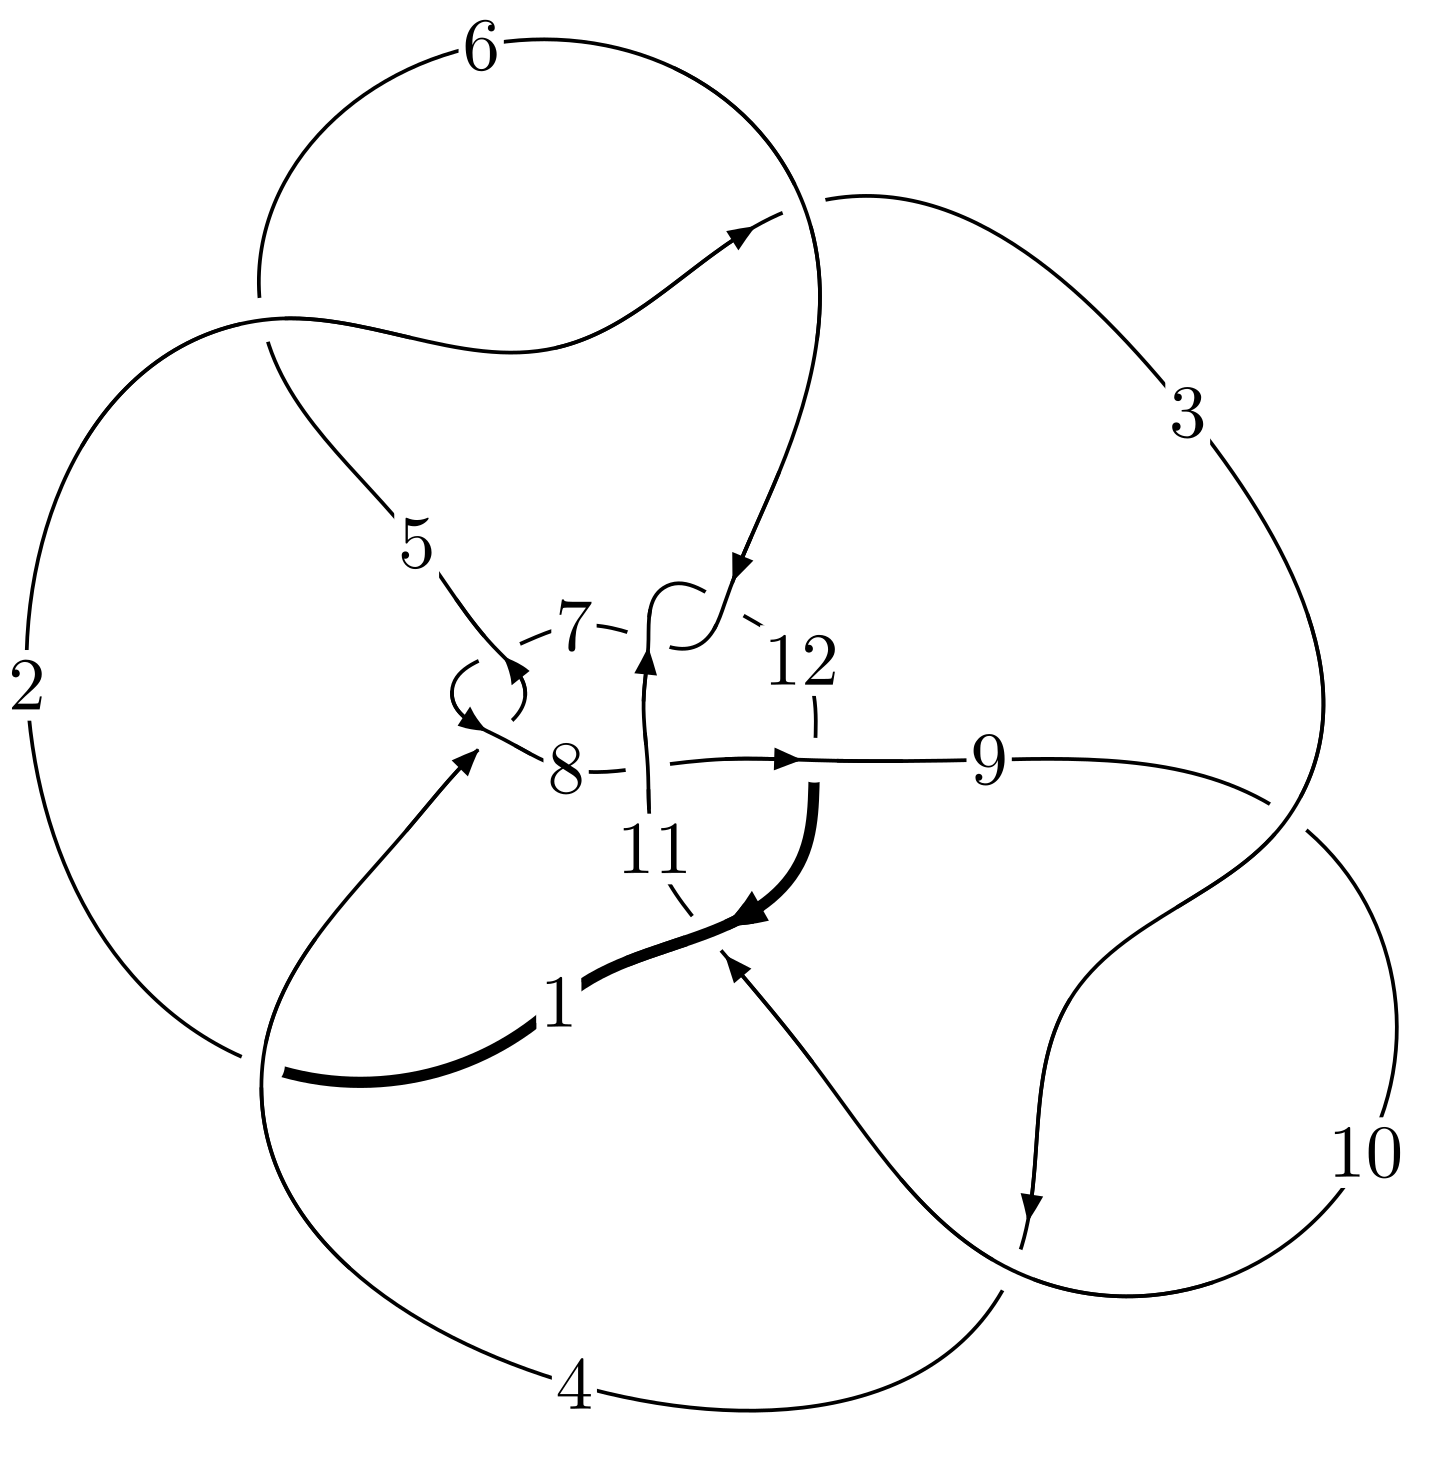
\includegraphics[width=112pt]{../../../GIT/diagram.site/Diagrams/png/2880_12n_0791.png}\\
\ \ \ A knot diagram\footnotemark}&
\allowdisplaybreaks
\textbf{Linearized knot diagam} \\
\cline{2-2}
 &
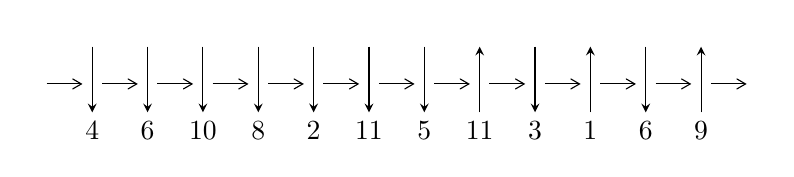
\begin{tikzpicture}[x=20pt, y=17pt]
	% nodes
	\node (C0) at (0, 0) {};
	\node (C1) at (1, 0) {};
	\node (C1U) at (1, +1) {};
	\node (C1D) at (1, -1) {4};

	\node (C2) at (2, 0) {};
	\node (C2U) at (2, +1) {};
	\node (C2D) at (2, -1) {6};

	\node (C3) at (3, 0) {};
	\node (C3U) at (3, +1) {};
	\node (C3D) at (3, -1) {10};

	\node (C4) at (4, 0) {};
	\node (C4U) at (4, +1) {};
	\node (C4D) at (4, -1) {8};

	\node (C5) at (5, 0) {};
	\node (C5U) at (5, +1) {};
	\node (C5D) at (5, -1) {2};

	\node (C6) at (6, 0) {};
	\node (C6U) at (6, +1) {};
	\node (C6D) at (6, -1) {11};

	\node (C7) at (7, 0) {};
	\node (C7U) at (7, +1) {};
	\node (C7D) at (7, -1) {5};

	\node (C8) at (8, 0) {};
	\node (C8U) at (8, +1) {};
	\node (C8D) at (8, -1) {11};

	\node (C9) at (9, 0) {};
	\node (C9U) at (9, +1) {};
	\node (C9D) at (9, -1) {3};

	\node (C10) at (10, 0) {};
	\node (C10U) at (10, +1) {};
	\node (C10D) at (10, -1) {1};

	\node (C11) at (11, 0) {};
	\node (C11U) at (11, +1) {};
	\node (C11D) at (11, -1) {6};

	\node (C12) at (12, 0) {};
	\node (C12U) at (12, +1) {};
	\node (C12D) at (12, -1) {9};
	\node (C13) at (13, 0) {};

	% arrows
	\draw[->,>={angle 60}]
	(C0) edge (C1) (C1) edge (C2) (C2) edge (C3) (C3) edge (C4) (C4) edge (C5) (C5) edge (C6) (C6) edge (C7) (C7) edge (C8) (C8) edge (C9) (C9) edge (C10) (C10) edge (C11) (C11) edge (C12) (C12) edge (C13) ;	\draw[->,>=stealth]
	(C1U) edge (C1D) (C2U) edge (C2D) (C3U) edge (C3D) (C4U) edge (C4D) (C5U) edge (C5D) (C6U) edge (C6D) (C7U) edge (C7D) (C8D) edge (C8U) (C9U) edge (C9D) (C10D) edge (C10U) (C11U) edge (C11D) (C12D) edge (C12U) ;
	\end{tikzpicture} \\
\hhline{~~} \\& 
\textbf{Solving Sequence} \\ \cline{2-2} 
 &
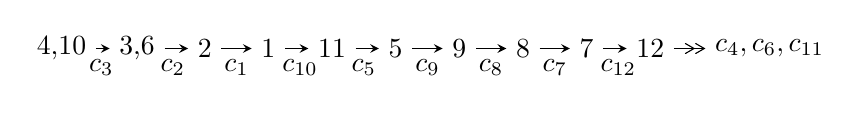
\begin{tikzpicture}[x=23pt, y=7pt]
	% node
	\node (A0) at (-1/8, 0) {4,10};
	\node (A1) at (17/16, 0) {3,6};
	\node (A2) at (17/8, 0) {2};
	\node (A3) at (25/8, 0) {1};
	\node (A4) at (33/8, 0) {11};
	\node (A5) at (41/8, 0) {5};
	\node (A6) at (49/8, 0) {9};
	\node (A7) at (57/8, 0) {8};
	\node (A8) at (65/8, 0) {7};
	\node (A9) at (73/8, 0) {12};
	\node (C1) at (1/2, -1) {$c_{3}$};
	\node (C2) at (13/8, -1) {$c_{2}$};
	\node (C3) at (21/8, -1) {$c_{1}$};
	\node (C4) at (29/8, -1) {$c_{10}$};
	\node (C5) at (37/8, -1) {$c_{5}$};
	\node (C6) at (45/8, -1) {$c_{9}$};
	\node (C7) at (53/8, -1) {$c_{8}$};
	\node (C8) at (61/8, -1) {$c_{7}$};
	\node (C9) at (69/8, -1) {$c_{12}$};
	\node (A10) at (11, 0) {$c_{4},c_{6},c_{11}$};

	% edge
	\draw[->,>=stealth]	
	(A0) edge (A1) (A1) edge (A2) (A2) edge (A3) (A3) edge (A4) (A4) edge (A5) (A5) edge (A6) (A6) edge (A7) (A7) edge (A8) (A8) edge (A9) ;
	\draw[->>,>={angle 60}]	
	(A9) edge (A10);
\end{tikzpicture} \\ 

\end{tabular} \\

\footnotetext{
The image of knot diagram is generated by the software ``\textbf{Draw programme}" developed by Andrew Bartholomew(\url{http://www.layer8.co.uk/maths/draw/index.htm\#Running-draw}), where we modified some parts for our purpose(\url{https://github.com/CATsTAILs/LinksPainter}).
}\phantom \\ \newline 
\centering \textbf{Ideals for irreducible components\footnotemark of $X_{\text{par}}$} 
 
\begin{align*}
I^u_{1}&=\langle 
3.33940\times10^{221} u^{77}+3.62622\times10^{220} u^{76}+\cdots+1.11812\times10^{223} b+2.16286\times10^{224},\\
\phantom{I^u_{1}}&\phantom{= \langle  }1.25797\times10^{224} u^{77}+2.59631\times10^{223} u^{76}+\cdots+7.97223\times10^{225} a-1.18016\times10^{227},\\
\phantom{I^u_{1}}&\phantom{= \langle  }u^{78}- u^{77}+\cdots+7307 u-713\rangle \\
I^u_{2}&=\langle 
9.42636\times10^{15} u^{31}-1.03650\times10^{16} u^{30}+\cdots+2.60834\times10^{15} b+8.63306\times10^{16},\\
\phantom{I^u_{2}}&\phantom{= \langle  }-8.60928\times10^{16} u^{31}+1.00029\times10^{17} u^{30}+\cdots+2.86917\times10^{16} a-1.03993\times10^{18},\\
\phantom{I^u_{2}}&\phantom{= \langle  }u^{32}-12 u^{30}+\cdots+14 u+11\rangle \\
\\
\end{align*}
\raggedright * 2 irreducible components of $\dim_{\mathbb{C}}=0$, with total 110 representations.\\
\footnotetext{All coefficients of polynomials are rational numbers. But the coefficients are sometimes approximated in decimal forms when there is not enough margin.}
\newpage
\renewcommand{\arraystretch}{1}
\centering \section*{I. $I^u_{1}= \langle 3.34\times10^{221} u^{77}+3.63\times10^{220} u^{76}+\cdots+1.12\times10^{223} b+2.16\times10^{224},\;1.26\times10^{224} u^{77}+2.60\times10^{223} u^{76}+\cdots+7.97\times10^{225} a-1.18\times10^{227},\;u^{78}- u^{77}+\cdots+7307 u-713 \rangle$}
\flushleft \textbf{(i) Arc colorings}\\
\begin{tabular}{m{7pt} m{180pt} m{7pt} m{180pt} }
\flushright $a_{4}=$&$\begin{pmatrix}1\\0\end{pmatrix}$ \\
\flushright $a_{10}=$&$\begin{pmatrix}0\\u\end{pmatrix}$ \\
\flushright $a_{3}=$&$\begin{pmatrix}1\\- u^2\end{pmatrix}$ \\
\flushright $a_{6}=$&$\begin{pmatrix}-0.0157793 u^{77}-0.00325669 u^{76}+\cdots-26.8738 u+14.8034\\-0.0298661 u^{77}-0.00324312 u^{76}+\cdots+175.664 u-19.3436\end{pmatrix}$ \\
\flushright $a_{2}=$&$\begin{pmatrix}0.0121080 u^{77}-0.0122585 u^{76}+\cdots-260.939 u+42.1759\\0.0127688 u^{77}+0.000485058 u^{76}+\cdots-101.992 u+11.9796\end{pmatrix}$ \\
\flushright $a_{1}=$&$\begin{pmatrix}0.0248767 u^{77}-0.0117734 u^{76}+\cdots-362.931 u+54.1555\\0.0127688 u^{77}+0.000485058 u^{76}+\cdots-101.992 u+11.9796\end{pmatrix}$ \\
\flushright $a_{11}=$&$\begin{pmatrix}0.0150625 u^{77}-0.0141531 u^{76}+\cdots-304.583 u+44.1204\\0.00161713 u^{77}+0.00303149 u^{76}+\cdots+21.4007 u-5.05900\end{pmatrix}$ \\
\flushright $a_{5}=$&$\begin{pmatrix}-0.117342 u^{77}+0.0172410 u^{76}+\cdots+835.872 u-90.0394\\-0.0229477 u^{77}-0.00152551 u^{76}+\cdots+164.335 u-20.6918\end{pmatrix}$ \\
\flushright $a_{9}=$&$\begin{pmatrix}u\\- u^3+u\end{pmatrix}$ \\
\flushright $a_{8}=$&$\begin{pmatrix}0.0594370 u^{77}-0.0231347 u^{76}+\cdots-617.741 u+82.9433\\0.00163959 u^{77}-0.00205736 u^{76}+\cdots-58.1641 u+9.02172\end{pmatrix}$ \\
\flushright $a_{7}=$&$\begin{pmatrix}-0.0839403 u^{77}+0.00200465 u^{76}+\cdots+589.203 u-61.4125\\-0.00229897 u^{77}-0.00218375 u^{76}+\cdots-22.8424 u+5.75187\end{pmatrix}$ \\
\flushright $a_{12}=$&$\begin{pmatrix}0.00354460 u^{77}-0.0181944 u^{76}+\cdots-257.161 u+43.8462\\0.0257467 u^{77}+0.00283761 u^{76}+\cdots-183.805 u+21.4583\end{pmatrix}$\\&\end{tabular}
\flushleft \textbf{(ii) Obstruction class $= -1$}\\~\\
\flushleft \textbf{(iii) Cusp Shapes $= 0.0607658 u^{77}-0.0336953 u^{76}+\cdots-399.330 u+14.9628$}\\~\\
\newpage\renewcommand{\arraystretch}{1}
\flushleft \textbf{(iv) u-Polynomials at the component}\newline \\
\begin{tabular}{m{50pt}|m{274pt}}
Crossings & \hspace{64pt}u-Polynomials at each crossing \\
\hline $$\begin{aligned}c_{1}\end{aligned}$$&$\begin{aligned}
&u^{78}-9 u^{77}+\cdots-30111 u-3476
\end{aligned}$\\
\hline $$\begin{aligned}c_{2},c_{5}\end{aligned}$$&$\begin{aligned}
&u^{78}+u^{77}+\cdots+25 u-1
\end{aligned}$\\
\hline $$\begin{aligned}c_{3},c_{9}\end{aligned}$$&$\begin{aligned}
&u^{78}- u^{77}+\cdots+7307 u-713
\end{aligned}$\\
\hline $$\begin{aligned}c_{4},c_{7}\end{aligned}$$&$\begin{aligned}
&u^{78}-5 u^{77}+\cdots+20 u-1
\end{aligned}$\\
\hline $$\begin{aligned}c_{6},c_{11}\end{aligned}$$&$\begin{aligned}
&u^{78}+3 u^{77}+\cdots-734300 u+685471
\end{aligned}$\\
\hline $$\begin{aligned}c_{8}\end{aligned}$$&$\begin{aligned}
&u^{78}+5 u^{77}+\cdots+107670903 u+34552577
\end{aligned}$\\
\hline $$\begin{aligned}c_{10}\end{aligned}$$&$\begin{aligned}
&u^{78}+u^{77}+\cdots+729 u+31
\end{aligned}$\\
\hline $$\begin{aligned}c_{12}\end{aligned}$$&$\begin{aligned}
&u^{78}-3 u^{77}+\cdots+5399717 u+801148
\end{aligned}$\\
\hline
\end{tabular}\\~\\
\newpage\renewcommand{\arraystretch}{1}
\flushleft \textbf{(v) Riley Polynomials at the component}\newline \\
\begin{tabular}{m{50pt}|m{274pt}}
Crossings & \hspace{64pt}Riley Polynomials at each crossing \\
\hline $$\begin{aligned}c_{1}\end{aligned}$$&$\begin{aligned}
&y^{78}-27 y^{77}+\cdots+17262383 y+12082576
\end{aligned}$\\
\hline $$\begin{aligned}c_{2},c_{5}\end{aligned}$$&$\begin{aligned}
&y^{78}-73 y^{77}+\cdots+105 y+1
\end{aligned}$\\
\hline $$\begin{aligned}c_{3},c_{9}\end{aligned}$$&$\begin{aligned}
&y^{78}-67 y^{77}+\cdots-15851373 y+508369
\end{aligned}$\\
\hline $$\begin{aligned}c_{4},c_{7}\end{aligned}$$&$\begin{aligned}
&y^{78}+17 y^{77}+\cdots-408 y+1
\end{aligned}$\\
\hline $$\begin{aligned}c_{6},c_{11}\end{aligned}$$&$\begin{aligned}
&y^{78}-83 y^{77}+\cdots-10360427562352 y+469870491841
\end{aligned}$\\
\hline $$\begin{aligned}c_{8}\end{aligned}$$&$\begin{aligned}
&y^{78}+69 y^{77}+\cdots-21520300962268511 y+1193880577340929
\end{aligned}$\\
\hline $$\begin{aligned}c_{10}\end{aligned}$$&$\begin{aligned}
&y^{78}+5 y^{77}+\cdots-120505 y+961
\end{aligned}$\\
\hline $$\begin{aligned}c_{12}\end{aligned}$$&$\begin{aligned}
&y^{78}+73 y^{77}+\cdots-7450965034177 y+641838117904
\end{aligned}$\\
\hline
\end{tabular}\\~\\
\newpage\flushleft \textbf{(vi) Complex Volumes and Cusp Shapes}
$$\begin{array}{c|c|c}  
\text{Solutions to }I^u_{1}& \I (\text{vol} + \sqrt{-1}CS) & \text{Cusp shape}\\
 \hline 
\begin{aligned}
u &= \phantom{-}0.942844 + 0.058139 I \\
a &= \phantom{-}0.387472 + 0.733615 I \\
b &= -0.195034 + 0.610856 I\end{aligned}
 & \phantom{-}3.47891 - 1.49180 I & -6.00000 + 0. I\phantom{ +0.000000I} \\ \hline\begin{aligned}
u &= \phantom{-}0.942844 - 0.058139 I \\
a &= \phantom{-}0.387472 - 0.733615 I \\
b &= -0.195034 - 0.610856 I\end{aligned}
 & \phantom{-}3.47891 + 1.49180 I & -6.00000 + 0. I\phantom{ +0.000000I} \\ \hline\begin{aligned}
u &= -0.233950 + 0.908933 I \\
a &= -0.417189 - 0.871468 I \\
b &= -0.705334 - 0.166427 I\end{aligned}
 & \phantom{-}2.67343 + 2.46581 I & -6.00000 - 7.69832 I \\ \hline\begin{aligned}
u &= -0.233950 - 0.908933 I \\
a &= -0.417189 + 0.871468 I \\
b &= -0.705334 + 0.166427 I\end{aligned}
 & \phantom{-}2.67343 - 2.46581 I & -6.00000 + 7.69832 I \\ \hline\begin{aligned}
u &= -1.052020 + 0.174510 I \\
a &= \phantom{-}0.301022 - 0.112833 I \\
b &= \phantom{-}0.098599 - 0.266687 I\end{aligned}
 & -2.28336 + 0.03067 I & \phantom{-0.000000 } 0 \\ \hline\begin{aligned}
u &= -1.052020 - 0.174510 I \\
a &= \phantom{-}0.301022 + 0.112833 I \\
b &= \phantom{-}0.098599 + 0.266687 I\end{aligned}
 & -2.28336 - 0.03067 I & \phantom{-0.000000 } 0 \\ \hline\begin{aligned}
u &= \phantom{-}0.985202 + 0.543560 I \\
a &= \phantom{-}0.344444 - 0.317962 I \\
b &= -0.725802 - 0.187739 I\end{aligned}
 & \phantom{-}1.16693 - 4.65623 I & \phantom{-0.000000 } 0 \\ \hline\begin{aligned}
u &= \phantom{-}0.985202 - 0.543560 I \\
a &= \phantom{-}0.344444 + 0.317962 I \\
b &= -0.725802 + 0.187739 I\end{aligned}
 & \phantom{-}1.16693 + 4.65623 I & \phantom{-0.000000 } 0 \\ \hline\begin{aligned}
u &= \phantom{-}0.512915 + 0.664507 I \\
a &= -0.019800 - 0.447055 I \\
b &= -0.502437 + 0.036527 I\end{aligned}
 & \phantom{-}2.57696 - 0.05718 I & -1.84410 - 0.26283 I \\ \hline\begin{aligned}
u &= \phantom{-}0.512915 - 0.664507 I \\
a &= -0.019800 + 0.447055 I \\
b &= -0.502437 - 0.036527 I\end{aligned}
 & \phantom{-}2.57696 + 0.05718 I & -1.84410 + 0.26283 I\\
 \hline 
 \end{array}$$\newpage$$\begin{array}{c|c|c}  
\text{Solutions to }I^u_{1}& \I (\text{vol} + \sqrt{-1}CS) & \text{Cusp shape}\\
 \hline 
\begin{aligned}
u &= -0.117457 + 0.796160 I \\
a &= \phantom{-}0.799606 + 0.362909 I \\
b &= \phantom{-}1.54042 + 0.31597 I\end{aligned}
 & -1.82800 - 1.56177 I & -11.06612 + 4.95728 I \\ \hline\begin{aligned}
u &= -0.117457 - 0.796160 I \\
a &= \phantom{-}0.799606 - 0.362909 I \\
b &= \phantom{-}1.54042 - 0.31597 I\end{aligned}
 & -1.82800 + 1.56177 I & -11.06612 - 4.95728 I \\ \hline\begin{aligned}
u &= \phantom{-}0.788310 + 0.067667 I \\
a &= \phantom{-}0.34762 + 1.53388 I \\
b &= -0.222137 + 0.211517 I\end{aligned}
 & \phantom{-}4.10212 + 0.95252 I & -6.69747 - 11.08186 I \\ \hline\begin{aligned}
u &= \phantom{-}0.788310 - 0.067667 I \\
a &= \phantom{-}0.34762 - 1.53388 I \\
b &= -0.222137 - 0.211517 I\end{aligned}
 & \phantom{-}4.10212 - 0.95252 I & -6.69747 + 11.08186 I \\ \hline\begin{aligned}
u &= -1.181570 + 0.296006 I \\
a &= -1.25923 - 1.88608 I \\
b &= \phantom{-}1.53208 + 1.70546 I\end{aligned}
 & -9.81204 + 5.88301 I & \phantom{-0.000000 } 0 \\ \hline\begin{aligned}
u &= -1.181570 - 0.296006 I \\
a &= -1.25923 + 1.88608 I \\
b &= \phantom{-}1.53208 - 1.70546 I\end{aligned}
 & -9.81204 - 5.88301 I & \phantom{-0.000000 } 0 \\ \hline\begin{aligned}
u &= \phantom{-}0.370228 + 0.671180 I \\
a &= \phantom{-}0.426280 - 0.076400 I \\
b &= -0.016730 - 0.393794 I\end{aligned}
 & \phantom{-}1.81907 + 1.89583 I & \phantom{-}1.064668 + 0.345602 I \\ \hline\begin{aligned}
u &= \phantom{-}0.370228 - 0.671180 I \\
a &= \phantom{-}0.426280 + 0.076400 I \\
b &= -0.016730 + 0.393794 I\end{aligned}
 & \phantom{-}1.81907 - 1.89583 I & \phantom{-}1.064668 - 0.345602 I \\ \hline\begin{aligned}
u &= -0.262253 + 0.715559 I \\
a &= -0.814627 + 0.211044 I \\
b &= \phantom{-}1.082170 - 0.442549 I\end{aligned}
 & -7.06075 - 2.20723 I & -7.08678 + 2.81313 I \\ \hline\begin{aligned}
u &= -0.262253 - 0.715559 I \\
a &= -0.814627 - 0.211044 I \\
b &= \phantom{-}1.082170 + 0.442549 I\end{aligned}
 & -7.06075 + 2.20723 I & -7.08678 - 2.81313 I\\
 \hline 
 \end{array}$$\newpage$$\begin{array}{c|c|c}  
\text{Solutions to }I^u_{1}& \I (\text{vol} + \sqrt{-1}CS) & \text{Cusp shape}\\
 \hline 
\begin{aligned}
u &= \phantom{-}1.115340 + 0.560449 I \\
a &= -0.169288 - 0.244756 I \\
b &= -0.165686 + 0.541919 I\end{aligned}
 & -0.34731 - 6.68579 I & \phantom{-0.000000 } 0 \\ \hline\begin{aligned}
u &= \phantom{-}1.115340 - 0.560449 I \\
a &= -0.169288 + 0.244756 I \\
b &= -0.165686 - 0.541919 I\end{aligned}
 & -0.34731 + 6.68579 I & \phantom{-0.000000 } 0 \\ \hline\begin{aligned}
u &= \phantom{-}1.228540 + 0.240197 I \\
a &= -0.702013 - 1.070830 I \\
b &= \phantom{-}0.51943 + 2.25418 I\end{aligned}
 & -6.10822 - 3.54460 I & \phantom{-0.000000 } 0 \\ \hline\begin{aligned}
u &= \phantom{-}1.228540 - 0.240197 I \\
a &= -0.702013 + 1.070830 I \\
b &= \phantom{-}0.51943 - 2.25418 I\end{aligned}
 & -6.10822 + 3.54460 I & \phantom{-0.000000 } 0 \\ \hline\begin{aligned}
u &= \phantom{-}1.262970 + 0.047018 I \\
a &= \phantom{-}1.55368 - 0.40771 I \\
b &= -1.53769 + 1.10929 I\end{aligned}
 & -3.54474 - 4.39179 I & \phantom{-0.000000 } 0 \\ \hline\begin{aligned}
u &= \phantom{-}1.262970 - 0.047018 I \\
a &= \phantom{-}1.55368 + 0.40771 I \\
b &= -1.53769 - 1.10929 I\end{aligned}
 & -3.54474 + 4.39179 I & \phantom{-0.000000 } 0 \\ \hline\begin{aligned}
u &= -1.191080 + 0.473505 I \\
a &= -0.103272 + 0.395239 I \\
b &= \phantom{-}0.250583 + 0.278590 I\end{aligned}
 & -0.35015 + 2.38063 I & \phantom{-0.000000 } 0 \\ \hline\begin{aligned}
u &= -1.191080 - 0.473505 I \\
a &= -0.103272 - 0.395239 I \\
b &= \phantom{-}0.250583 - 0.278590 I\end{aligned}
 & -0.35015 - 2.38063 I & \phantom{-0.000000 } 0 \\ \hline\begin{aligned}
u &= -1.277390 + 0.110090 I \\
a &= -2.20740 - 0.08937 I \\
b &= \phantom{-}1.97105 - 0.56101 I\end{aligned}
 & -4.35623 + 3.03953 I & \phantom{-0.000000 } 0 \\ \hline\begin{aligned}
u &= -1.277390 - 0.110090 I \\
a &= -2.20740 + 0.08937 I \\
b &= \phantom{-}1.97105 + 0.56101 I\end{aligned}
 & -4.35623 - 3.03953 I & \phantom{-0.000000 } 0\\
 \hline 
 \end{array}$$\newpage$$\begin{array}{c|c|c}  
\text{Solutions to }I^u_{1}& \I (\text{vol} + \sqrt{-1}CS) & \text{Cusp shape}\\
 \hline 
\begin{aligned}
u &= -1.291280 + 0.159820 I \\
a &= \phantom{-}1.98881 + 1.23832 I \\
b &= -2.27722 - 1.32574 I\end{aligned}
 & -11.24160 - 1.94282 I & \phantom{-0.000000 } 0 \\ \hline\begin{aligned}
u &= -1.291280 - 0.159820 I \\
a &= \phantom{-}1.98881 - 1.23832 I \\
b &= -2.27722 + 1.32574 I\end{aligned}
 & -11.24160 + 1.94282 I & \phantom{-0.000000 } 0 \\ \hline\begin{aligned}
u &= \phantom{-}1.317320 + 0.121357 I \\
a &= \phantom{-}0.177970 + 1.254660 I \\
b &= -0.06318 - 2.60422 I\end{aligned}
 & -5.17676 + 4.17039 I & \phantom{-0.000000 } 0 \\ \hline\begin{aligned}
u &= \phantom{-}1.317320 - 0.121357 I \\
a &= \phantom{-}0.177970 - 1.254660 I \\
b &= -0.06318 + 2.60422 I\end{aligned}
 & -5.17676 - 4.17039 I & \phantom{-0.000000 } 0 \\ \hline\begin{aligned}
u &= \phantom{-}1.263750 + 0.446195 I \\
a &= \phantom{-}1.94787 - 0.98680 I \\
b &= -2.78785 - 0.16314 I\end{aligned}
 & -1.79519 - 7.98956 I & \phantom{-0.000000 } 0 \\ \hline\begin{aligned}
u &= \phantom{-}1.263750 - 0.446195 I \\
a &= \phantom{-}1.94787 + 0.98680 I \\
b &= -2.78785 + 0.16314 I\end{aligned}
 & -1.79519 + 7.98956 I & \phantom{-0.000000 } 0 \\ \hline\begin{aligned}
u &= \phantom{-}1.333270 + 0.154113 I \\
a &= -2.17809 - 0.01089 I \\
b &= \phantom{-}2.72516 + 0.87884 I\end{aligned}
 & -6.73250 - 1.36559 I & \phantom{-0.000000 } 0 \\ \hline\begin{aligned}
u &= \phantom{-}1.333270 - 0.154113 I \\
a &= -2.17809 + 0.01089 I \\
b &= \phantom{-}2.72516 - 0.87884 I\end{aligned}
 & -6.73250 + 1.36559 I & \phantom{-0.000000 } 0 \\ \hline\begin{aligned}
u &= -0.247106 + 1.366830 I \\
a &= \phantom{-}0.286312 + 0.222429 I \\
b &= \phantom{-}1.88034 + 0.30072 I\end{aligned}
 & -8.58231 + 2.86666 I & \phantom{-0.000000 } 0 \\ \hline\begin{aligned}
u &= -0.247106 - 1.366830 I \\
a &= \phantom{-}0.286312 - 0.222429 I \\
b &= \phantom{-}1.88034 - 0.30072 I\end{aligned}
 & -8.58231 - 2.86666 I & \phantom{-0.000000 } 0\\
 \hline 
 \end{array}$$\newpage$$\begin{array}{c|c|c}  
\text{Solutions to }I^u_{1}& \I (\text{vol} + \sqrt{-1}CS) & \text{Cusp shape}\\
 \hline 
\begin{aligned}
u &= -0.146469 + 0.591338 I \\
a &= \phantom{-}1.169670 - 0.079543 I \\
b &= -1.066960 + 0.481680 I\end{aligned}
 & -7.60805 + 4.49193 I & -8.55555 - 2.21842 I \\ \hline\begin{aligned}
u &= -0.146469 - 0.591338 I \\
a &= \phantom{-}1.169670 + 0.079543 I \\
b &= -1.066960 - 0.481680 I\end{aligned}
 & -7.60805 - 4.49193 I & -8.55555 + 2.21842 I \\ \hline\begin{aligned}
u &= \phantom{-}0.297121 + 1.371380 I \\
a &= -0.371698 - 0.504760 I \\
b &= -2.17012 - 0.07122 I\end{aligned}
 & \phantom{-}1.90547 + 2.10501 I & \phantom{-0.000000 } 0 \\ \hline\begin{aligned}
u &= \phantom{-}0.297121 - 1.371380 I \\
a &= -0.371698 + 0.504760 I \\
b &= -2.17012 + 0.07122 I\end{aligned}
 & \phantom{-}1.90547 - 2.10501 I & \phantom{-0.000000 } 0 \\ \hline\begin{aligned}
u &= -0.266211 + 1.384610 I \\
a &= -0.228160 - 0.202664 I \\
b &= -1.84539 - 0.24540 I\end{aligned}
 & -7.80585 + 10.06730 I & \phantom{-0.000000 } 0 \\ \hline\begin{aligned}
u &= -0.266211 - 1.384610 I \\
a &= -0.228160 + 0.202664 I \\
b &= -1.84539 + 0.24540 I\end{aligned}
 & -7.80585 - 10.06730 I & \phantom{-0.000000 } 0 \\ \hline\begin{aligned}
u &= -1.399680 + 0.173379 I \\
a &= \phantom{-}0.334409 - 0.519138 I \\
b &= -0.111903 - 0.458529 I\end{aligned}
 & -8.31581 + 1.61430 I & \phantom{-0.000000 } 0 \\ \hline\begin{aligned}
u &= -1.399680 - 0.173379 I \\
a &= \phantom{-}0.334409 + 0.519138 I \\
b &= -0.111903 + 0.458529 I\end{aligned}
 & -8.31581 - 1.61430 I & \phantom{-0.000000 } 0 \\ \hline\begin{aligned}
u &= -1.37866 + 0.36295 I \\
a &= -1.64976 - 0.50953 I \\
b &= \phantom{-}1.80542 - 0.82492 I\end{aligned}
 & -6.03995 + 5.96238 I & \phantom{-0.000000 } 0 \\ \hline\begin{aligned}
u &= -1.37866 - 0.36295 I \\
a &= -1.64976 + 0.50953 I \\
b &= \phantom{-}1.80542 + 0.82492 I\end{aligned}
 & -6.03995 - 5.96238 I & \phantom{-0.000000 } 0\\
 \hline 
 \end{array}$$\newpage$$\begin{array}{c|c|c}  
\text{Solutions to }I^u_{1}& \I (\text{vol} + \sqrt{-1}CS) & \text{Cusp shape}\\
 \hline 
\begin{aligned}
u &= \phantom{-}1.40559 + 0.25706 I \\
a &= \phantom{-}1.64134 - 0.25262 I \\
b &= -1.55258 + 0.17099 I\end{aligned}
 & -12.6770 - 7.6946 I & \phantom{-0.000000 } 0 \\ \hline\begin{aligned}
u &= \phantom{-}1.40559 - 0.25706 I \\
a &= \phantom{-}1.64134 + 0.25262 I \\
b &= -1.55258 - 0.17099 I\end{aligned}
 & -12.6770 + 7.6946 I & \phantom{-0.000000 } 0 \\ \hline\begin{aligned}
u &= -1.45079 + 0.18447 I \\
a &= -0.289984 + 0.565798 I \\
b &= \phantom{-}0.120076 + 0.470255 I\end{aligned}
 & -7.53186 + 8.23802 I & \phantom{-0.000000 } 0 \\ \hline\begin{aligned}
u &= -1.45079 - 0.18447 I \\
a &= -0.289984 - 0.565798 I \\
b &= \phantom{-}0.120076 - 0.470255 I\end{aligned}
 & -7.53186 - 8.23802 I & \phantom{-0.000000 } 0 \\ \hline\begin{aligned}
u &= \phantom{-}0.210864 + 0.491337 I \\
a &= \phantom{-}1.94925 + 1.15029 I \\
b &= \phantom{-}0.515472 - 0.844495 I\end{aligned}
 & -3.08975 + 0.76544 I & -5.09780 - 0.03360 I \\ \hline\begin{aligned}
u &= \phantom{-}0.210864 - 0.491337 I \\
a &= \phantom{-}1.94925 - 1.15029 I \\
b &= \phantom{-}0.515472 + 0.844495 I\end{aligned}
 & -3.08975 - 0.76544 I & -5.09780 + 0.03360 I \\ \hline\begin{aligned}
u &= -0.357502 + 0.389914 I \\
a &= \phantom{-}1.057850 - 0.269178 I \\
b &= \phantom{-}1.216960 + 0.412368 I\end{aligned}
 & -1.18445 - 1.39735 I & -10.38498 - 7.63627 I \\ \hline\begin{aligned}
u &= -0.357502 - 0.389914 I \\
a &= \phantom{-}1.057850 + 0.269178 I \\
b &= \phantom{-}1.216960 - 0.412368 I\end{aligned}
 & -1.18445 + 1.39735 I & -10.38498 + 7.63627 I \\ \hline\begin{aligned}
u &= \phantom{-}1.45944 + 0.24660 I \\
a &= -1.60374 + 0.25242 I \\
b &= \phantom{-}1.67036 - 0.13168 I\end{aligned}
 & -12.74980 - 1.29840 I & \phantom{-0.000000 } 0 \\ \hline\begin{aligned}
u &= \phantom{-}1.45944 - 0.24660 I \\
a &= -1.60374 - 0.25242 I \\
b &= \phantom{-}1.67036 + 0.13168 I\end{aligned}
 & -12.74980 + 1.29840 I & \phantom{-0.000000 } 0\\
 \hline 
 \end{array}$$\newpage$$\begin{array}{c|c|c}  
\text{Solutions to }I^u_{1}& \I (\text{vol} + \sqrt{-1}CS) & \text{Cusp shape}\\
 \hline 
\begin{aligned}
u &= -1.47987 + 0.09429 I \\
a &= \phantom{-}1.64800 - 0.11539 I \\
b &= -1.92274 + 0.85333 I\end{aligned}
 & -6.22918 + 4.98031 I & \phantom{-0.000000 } 0 \\ \hline\begin{aligned}
u &= -1.47987 - 0.09429 I \\
a &= \phantom{-}1.64800 + 0.11539 I \\
b &= -1.92274 - 0.85333 I\end{aligned}
 & -6.22918 - 4.98031 I & \phantom{-0.000000 } 0 \\ \hline\begin{aligned}
u &= \phantom{-}0.268582 + 0.388279 I \\
a &= -2.50694 - 2.55703 I \\
b &= -0.609144 + 1.104730 I\end{aligned}
 & -1.75519 - 5.95991 I & -1.96592 + 6.04253 I \\ \hline\begin{aligned}
u &= \phantom{-}0.268582 - 0.388279 I \\
a &= -2.50694 + 2.55703 I \\
b &= -0.609144 - 1.104730 I\end{aligned}
 & -1.75519 + 5.95991 I & -1.96592 - 6.04253 I \\ \hline\begin{aligned}
u &= -0.421212\phantom{ +0.000000I} \\
a &= \phantom{-}0.897582\phantom{ +0.000000I} \\
b &= \phantom{-}0.341691\phantom{ +0.000000I}\end{aligned}
 & -0.747108\phantom{ +0.000000I} & -13.2570\phantom{ +0.000000I} \\ \hline\begin{aligned}
u &= \phantom{-}1.58306\phantom{ +0.000000I} \\
a &= -1.63258\phantom{ +0.000000I} \\
b &= \phantom{-}2.46027\phantom{ +0.000000I}\end{aligned}
 & -8.82351\phantom{ +0.000000I} & \phantom{-0.000000 } 0 \\ \hline\begin{aligned}
u &= -1.59892 + 0.25190 I \\
a &= \phantom{-}1.392980 + 0.180687 I \\
b &= -1.91042 + 0.74588 I\end{aligned}
 & -5.56562 + 3.33736 I & \phantom{-0.000000 } 0 \\ \hline\begin{aligned}
u &= -1.59892 - 0.25190 I \\
a &= \phantom{-}1.392980 - 0.180687 I \\
b &= -1.91042 - 0.74588 I\end{aligned}
 & -5.56562 - 3.33736 I & \phantom{-0.000000 } 0 \\ \hline\begin{aligned}
u &= \phantom{-}1.53550 + 0.51590 I \\
a &= -1.52077 + 0.57665 I \\
b &= \phantom{-}2.45062 + 0.56733 I\end{aligned}
 & -14.3064 - 9.3860 I & \phantom{-0.000000 } 0 \\ \hline\begin{aligned}
u &= \phantom{-}1.53550 - 0.51590 I \\
a &= -1.52077 - 0.57665 I \\
b &= \phantom{-}2.45062 - 0.56733 I\end{aligned}
 & -14.3064 + 9.3860 I & \phantom{-0.000000 } 0\\
 \hline 
 \end{array}$$\newpage$$\begin{array}{c|c|c}  
\text{Solutions to }I^u_{1}& \I (\text{vol} + \sqrt{-1}CS) & \text{Cusp shape}\\
 \hline 
\begin{aligned}
u &= \phantom{-}1.54978 + 0.53968 I \\
a &= \phantom{-}1.48248 - 0.57690 I \\
b &= -2.38130 - 0.59597 I\end{aligned}
 & -13.5587 - 16.7600 I & \phantom{-0.000000 } 0 \\ \hline\begin{aligned}
u &= \phantom{-}1.54978 - 0.53968 I \\
a &= \phantom{-}1.48248 + 0.57690 I \\
b &= -2.38130 + 0.59597 I\end{aligned}
 & -13.5587 + 16.7600 I & \phantom{-0.000000 } 0 \\ \hline\begin{aligned}
u &= \phantom{-}0.267828 + 0.052884 I \\
a &= \phantom{-}0.09300 - 3.41499 I \\
b &= -1.013240 - 0.178283 I\end{aligned}
 & -0.14166 - 4.08705 I & -7.04533 + 7.48783 I \\ \hline\begin{aligned}
u &= \phantom{-}0.267828 - 0.052884 I \\
a &= \phantom{-}0.09300 + 3.41499 I \\
b &= -1.013240 + 0.178283 I\end{aligned}
 & -0.14166 + 4.08705 I & -7.04533 - 7.48783 I \\ \hline\begin{aligned}
u &= -1.58752 + 0.74757 I \\
a &= -1.048890 - 0.614073 I \\
b &= \phantom{-}1.92049 - 1.18239 I\end{aligned}
 & -12.66830 + 5.03933 I & \phantom{-0.000000 } 0 \\ \hline\begin{aligned}
u &= -1.58752 - 0.74757 I \\
a &= -1.048890 + 0.614073 I \\
b &= \phantom{-}1.92049 + 1.18239 I\end{aligned}
 & -12.66830 - 5.03933 I & \phantom{-0.000000 } 0 \\ \hline\begin{aligned}
u &= -1.67659 + 0.87833 I \\
a &= \phantom{-}0.915811 + 0.565877 I \\
b &= -1.91733 + 1.36586 I\end{aligned}
 & -11.65830 - 1.69347 I & \phantom{-0.000000 } 0 \\ \hline\begin{aligned}
u &= -1.67659 - 0.87833 I \\
a &= \phantom{-}0.915811 - 0.565877 I \\
b &= -1.91733 - 1.36586 I\end{aligned}
 & -11.65830 + 1.69347 I & \phantom{-0.000000 } 0\\
 \hline 
 \end{array}$$\newpage\newpage\renewcommand{\arraystretch}{1}
\centering \section*{II. $I^u_{2}= \langle 9.43\times10^{15} u^{31}-1.04\times10^{16} u^{30}+\cdots+2.61\times10^{15} b+8.63\times10^{16},\;-8.61\times10^{16} u^{31}+1.00\times10^{17} u^{30}+\cdots+2.87\times10^{16} a-1.04\times10^{18},\;u^{32}-12 u^{30}+\cdots+14 u+11 \rangle$}
\flushleft \textbf{(i) Arc colorings}\\
\begin{tabular}{m{7pt} m{180pt} m{7pt} m{180pt} }
\flushright $a_{4}=$&$\begin{pmatrix}1\\0\end{pmatrix}$ \\
\flushright $a_{10}=$&$\begin{pmatrix}0\\u\end{pmatrix}$ \\
\flushright $a_{3}=$&$\begin{pmatrix}1\\- u^2\end{pmatrix}$ \\
\flushright $a_{6}=$&$\begin{pmatrix}3.00062 u^{31}-3.48635 u^{30}+\cdots+16.9894 u+36.2451\\-3.61394 u^{31}+3.97380 u^{30}+\cdots-9.33313 u-33.0980\end{pmatrix}$ \\
\flushright $a_{2}=$&$\begin{pmatrix}0.673654 u^{31}-0.202721 u^{30}+\cdots-1.38111 u+6.42284\\0.436104 u^{31}-0.802754 u^{30}+\cdots+4.55569 u+3.93941\end{pmatrix}$ \\
\flushright $a_{1}=$&$\begin{pmatrix}1.10976 u^{31}-1.00548 u^{30}+\cdots+3.17457 u+10.3622\\0.436104 u^{31}-0.802754 u^{30}+\cdots+4.55569 u+3.93941\end{pmatrix}$ \\
\flushright $a_{11}=$&$\begin{pmatrix}-0.551853 u^{31}+1.15430 u^{30}+\cdots-4.09676 u-14.1990\\-0.260882 u^{31}+0.703792 u^{30}+\cdots-1.69474 u+0.574746\end{pmatrix}$ \\
\flushright $a_{5}=$&$\begin{pmatrix}2.29143 u^{31}-3.63005 u^{30}+\cdots+35.4371 u+40.5356\\-3.03963 u^{31}+3.45383 u^{30}+\cdots-7.45780 u-30.2115\end{pmatrix}$ \\
\flushright $a_{9}=$&$\begin{pmatrix}u\\- u^3+u\end{pmatrix}$ \\
\flushright $a_{8}=$&$\begin{pmatrix}0.227355 u^{31}-2.01232 u^{30}+\cdots+5.94324 u+7.33651\\-1.19027 u^{31}+1.68925 u^{30}+\cdots-11.2608 u-16.4565\end{pmatrix}$ \\
\flushright $a_{7}=$&$\begin{pmatrix}3.83119 u^{31}-3.80169 u^{30}+\cdots-5.28595 u+35.2770\\-4.36810 u^{31}+4.86030 u^{30}+\cdots-16.0382 u-45.6150\end{pmatrix}$ \\
\flushright $a_{12}=$&$\begin{pmatrix}-0.592703 u^{31}+1.96262 u^{30}+\cdots-9.25022 u-6.20976\\2.14537 u^{31}-3.17011 u^{30}+\cdots+14.9572 u+20.0165\end{pmatrix}$\\&\end{tabular}
\flushleft \textbf{(ii) Obstruction class $= 1$}\\~\\
\flushleft \textbf{(iii) Cusp Shapes $= -\frac{8803823690177608}{2608335035160577} u^{31}+\frac{27671018694520353}{2608335035160577} u^{30}+\cdots-\frac{228493900103964694}{2608335035160577} u-\frac{259489611336058185}{2608335035160577}$}\\~\\
\newpage\renewcommand{\arraystretch}{1}
\flushleft \textbf{(iv) u-Polynomials at the component}\newline \\
\begin{tabular}{m{50pt}|m{274pt}}
Crossings & \hspace{64pt}u-Polynomials at each crossing \\
\hline $$\begin{aligned}c_{1}\end{aligned}$$&$\begin{aligned}
&u^{32}-4 u^{31}+\cdots-60 u+9
\end{aligned}$\\
\hline $$\begin{aligned}c_{2}\end{aligned}$$&$\begin{aligned}
&u^{32}-9 u^{30}+\cdots-2 u+1
\end{aligned}$\\
\hline $$\begin{aligned}c_{3}\end{aligned}$$&$\begin{aligned}
&u^{32}-12 u^{30}+\cdots+14 u+11
\end{aligned}$\\
\hline $$\begin{aligned}c_{4}\end{aligned}$$&$\begin{aligned}
&u^{32}-8 u^{31}+\cdots-7 u+1
\end{aligned}$\\
\hline $$\begin{aligned}c_{5}\end{aligned}$$&$\begin{aligned}
&u^{32}-9 u^{30}+\cdots+2 u+1
\end{aligned}$\\
\hline $$\begin{aligned}c_{6}\end{aligned}$$&$\begin{aligned}
&u^{32}-2 u^{30}+\cdots+21 u+11
\end{aligned}$\\
\hline $$\begin{aligned}c_{7}\end{aligned}$$&$\begin{aligned}
&u^{32}+8 u^{31}+\cdots+7 u+1
\end{aligned}$\\
\hline $$\begin{aligned}c_{8}\end{aligned}$$&$\begin{aligned}
&u^{32}+4 u^{30}+\cdots+104 u+31
\end{aligned}$\\
\hline $$\begin{aligned}c_{9}\end{aligned}$$&$\begin{aligned}
&u^{32}-12 u^{30}+\cdots-14 u+11
\end{aligned}$\\
\hline $$\begin{aligned}c_{10}\end{aligned}$$&$\begin{aligned}
&u^{32}+16 u^{31}+\cdots+4 u+1
\end{aligned}$\\
\hline $$\begin{aligned}c_{11}\end{aligned}$$&$\begin{aligned}
&u^{32}-2 u^{30}+\cdots-21 u+11
\end{aligned}$\\
\hline $$\begin{aligned}c_{12}\end{aligned}$$&$\begin{aligned}
&u^{32}+4 u^{31}+\cdots-53 u+5
\end{aligned}$\\
\hline
\end{tabular}\\~\\
\newpage\renewcommand{\arraystretch}{1}
\flushleft \textbf{(v) Riley Polynomials at the component}\newline \\
\begin{tabular}{m{50pt}|m{274pt}}
Crossings & \hspace{64pt}Riley Polynomials at each crossing \\
\hline $$\begin{aligned}c_{1}\end{aligned}$$&$\begin{aligned}
&y^{32}-8 y^{30}+\cdots+684 y+81
\end{aligned}$\\
\hline $$\begin{aligned}c_{2},c_{5}\end{aligned}$$&$\begin{aligned}
&y^{32}-18 y^{31}+\cdots-14 y+1
\end{aligned}$\\
\hline $$\begin{aligned}c_{3},c_{9}\end{aligned}$$&$\begin{aligned}
&y^{32}-24 y^{31}+\cdots-1164 y+121
\end{aligned}$\\
\hline $$\begin{aligned}c_{4},c_{7}\end{aligned}$$&$\begin{aligned}
&y^{32}+12 y^{31}+\cdots+29 y+1
\end{aligned}$\\
\hline $$\begin{aligned}c_{6},c_{11}\end{aligned}$$&$\begin{aligned}
&y^{32}-4 y^{31}+\cdots+593 y+121
\end{aligned}$\\
\hline $$\begin{aligned}c_{8}\end{aligned}$$&$\begin{aligned}
&y^{32}+8 y^{31}+\cdots-5794 y+961
\end{aligned}$\\
\hline $$\begin{aligned}c_{10}\end{aligned}$$&$\begin{aligned}
&y^{32}-8 y^{31}+\cdots-8 y+1
\end{aligned}$\\
\hline $$\begin{aligned}c_{12}\end{aligned}$$&$\begin{aligned}
&y^{32}+16 y^{31}+\cdots-229 y+25
\end{aligned}$\\
\hline
\end{tabular}\\~\\
\newpage\flushleft \textbf{(vi) Complex Volumes and Cusp Shapes}
$$\begin{array}{c|c|c}  
\text{Solutions to }I^u_{2}& \I (\text{vol} + \sqrt{-1}CS) & \text{Cusp shape}\\
 \hline 
\begin{aligned}
u &= \phantom{-}0.608550 + 0.702570 I \\
a &= \phantom{-}0.054998 - 0.773982 I \\
b &= \phantom{-}0.028720 - 0.337814 I\end{aligned}
 & \phantom{-}1.10440 + 2.37787 I & -8.44125 - 4.16468 I \\ \hline\begin{aligned}
u &= \phantom{-}0.608550 - 0.702570 I \\
a &= \phantom{-}0.054998 + 0.773982 I \\
b &= \phantom{-}0.028720 + 0.337814 I\end{aligned}
 & \phantom{-}1.10440 - 2.37787 I & -8.44125 + 4.16468 I \\ \hline\begin{aligned}
u &= \phantom{-}0.393505 + 1.055530 I \\
a &= -0.378271 + 0.727602 I \\
b &= -0.564637 + 0.479550 I\end{aligned}
 & \phantom{-}2.95553 - 1.85219 I & -2.71010 - 2.33872 I \\ \hline\begin{aligned}
u &= \phantom{-}0.393505 - 1.055530 I \\
a &= -0.378271 - 0.727602 I \\
b &= -0.564637 - 0.479550 I\end{aligned}
 & \phantom{-}2.95553 + 1.85219 I & -2.71010 + 2.33872 I \\ \hline\begin{aligned}
u &= \phantom{-}1.149900 + 0.127905 I \\
a &= -0.126713 - 0.886278 I \\
b &= \phantom{-}0.029846 - 0.370064 I\end{aligned}
 & \phantom{-}2.90185 - 1.95756 I & -10.84834 + 6.93834 I \\ \hline\begin{aligned}
u &= \phantom{-}1.149900 - 0.127905 I \\
a &= -0.126713 + 0.886278 I \\
b &= \phantom{-}0.029846 + 0.370064 I\end{aligned}
 & \phantom{-}2.90185 + 1.95756 I & -10.84834 - 6.93834 I \\ \hline\begin{aligned}
u &= \phantom{-}0.792279 + 0.213841 I \\
a &= -0.257736 - 1.275920 I \\
b &= -0.020489 - 0.337783 I\end{aligned}
 & \phantom{-}4.30341 + 0.61589 I & \phantom{-}4.66315 + 6.19858 I \\ \hline\begin{aligned}
u &= \phantom{-}0.792279 - 0.213841 I \\
a &= -0.257736 + 1.275920 I \\
b &= -0.020489 + 0.337783 I\end{aligned}
 & \phantom{-}4.30341 - 0.61589 I & \phantom{-}4.66315 - 6.19858 I \\ \hline\begin{aligned}
u &= \phantom{-}1.123130 + 0.364207 I \\
a &= -1.00348 + 1.50445 I \\
b &= \phantom{-}0.903409 - 1.071170 I\end{aligned}
 & -9.60306 - 5.39034 I & -9.79295 - 0.61492 I \\ \hline\begin{aligned}
u &= \phantom{-}1.123130 - 0.364207 I \\
a &= -1.00348 - 1.50445 I \\
b &= \phantom{-}0.903409 + 1.071170 I\end{aligned}
 & -9.60306 + 5.39034 I & -9.79295 + 0.61492 I\\
 \hline 
 \end{array}$$\newpage$$\begin{array}{c|c|c}  
\text{Solutions to }I^u_{2}& \I (\text{vol} + \sqrt{-1}CS) & \text{Cusp shape}\\
 \hline 
\begin{aligned}
u &= \phantom{-}1.062610 + 0.540756 I \\
a &= -0.301171 + 0.165537 I \\
b &= -0.006583 - 0.183056 I\end{aligned}
 & -0.34395 - 7.11061 I & -6.1757 + 16.1016 I \\ \hline\begin{aligned}
u &= \phantom{-}1.062610 - 0.540756 I \\
a &= -0.301171 - 0.165537 I \\
b &= -0.006583 + 0.183056 I\end{aligned}
 & -0.34395 + 7.11061 I & -6.1757 - 16.1016 I \\ \hline\begin{aligned}
u &= -0.731631 + 0.286301 I \\
a &= \phantom{-}0.52628 - 1.91649 I \\
b &= \phantom{-}1.094140 + 0.871235 I\end{aligned}
 & -4.27035 - 0.78775 I & -13.76747 + 0.79111 I \\ \hline\begin{aligned}
u &= -0.731631 - 0.286301 I \\
a &= \phantom{-}0.52628 + 1.91649 I \\
b &= \phantom{-}1.094140 - 0.871235 I\end{aligned}
 & -4.27035 + 0.78775 I & -13.76747 - 0.79111 I \\ \hline\begin{aligned}
u &= -0.770679 + 0.148242 I \\
a &= \phantom{-}0.08527 + 3.02934 I \\
b &= -1.05799 - 1.31030 I\end{aligned}
 & -2.61922 + 5.83665 I & -12.12805 - 5.23486 I \\ \hline\begin{aligned}
u &= -0.770679 - 0.148242 I \\
a &= \phantom{-}0.08527 - 3.02934 I \\
b &= -1.05799 + 1.31030 I\end{aligned}
 & -2.61922 - 5.83665 I & -12.12805 + 5.23486 I \\ \hline\begin{aligned}
u &= \phantom{-}1.068010 + 0.613139 I \\
a &= -0.080989 - 0.362274 I \\
b &= \phantom{-}0.291002 + 0.024258 I\end{aligned}
 & \phantom{-}0.84523 - 3.87440 I & -7.28635 + 0.99100 I \\ \hline\begin{aligned}
u &= \phantom{-}1.068010 - 0.613139 I \\
a &= -0.080989 + 0.362274 I \\
b &= \phantom{-}0.291002 - 0.024258 I\end{aligned}
 & \phantom{-}0.84523 + 3.87440 I & -7.28635 - 0.99100 I \\ \hline\begin{aligned}
u &= -0.455603 + 1.225610 I \\
a &= -0.367004 + 0.445859 I \\
b &= -2.03913 - 0.37515 I\end{aligned}
 & \phantom{-}2.13581 - 2.36751 I & -0.13711 + 10.90887 I \\ \hline\begin{aligned}
u &= -0.455603 - 1.225610 I \\
a &= -0.367004 - 0.445859 I \\
b &= -2.03913 + 0.37515 I\end{aligned}
 & \phantom{-}2.13581 + 2.36751 I & -0.13711 - 10.90887 I\\
 \hline 
 \end{array}$$\newpage$$\begin{array}{c|c|c}  
\text{Solutions to }I^u_{2}& \I (\text{vol} + \sqrt{-1}CS) & \text{Cusp shape}\\
 \hline 
\begin{aligned}
u &= -1.311760 + 0.096882 I \\
a &= -1.85773 + 0.62801 I \\
b &= \phantom{-}2.09422 - 1.84300 I\end{aligned}
 & -6.92946 + 2.50095 I & -15.7221 - 2.9652 I \\ \hline\begin{aligned}
u &= -1.311760 - 0.096882 I \\
a &= -1.85773 - 0.62801 I \\
b &= \phantom{-}2.09422 + 1.84300 I\end{aligned}
 & -6.92946 - 2.50095 I & -15.7221 + 2.9652 I \\ \hline\begin{aligned}
u &= -1.326920 + 0.040818 I \\
a &= \phantom{-}0.862918 + 1.085500 I \\
b &= -1.10833 - 2.42545 I\end{aligned}
 & -5.10653 + 5.11428 I & -11.6019 - 9.0253 I \\ \hline\begin{aligned}
u &= -1.326920 - 0.040818 I \\
a &= \phantom{-}0.862918 - 1.085500 I \\
b &= -1.10833 + 2.42545 I\end{aligned}
 & -5.10653 - 5.11428 I & -11.6019 + 9.0253 I \\ \hline\begin{aligned}
u &= -1.286370 + 0.411422 I \\
a &= \phantom{-}1.96528 + 0.76818 I \\
b &= -2.57628 + 0.34784 I\end{aligned}
 & -1.23130 + 7.74404 I & -2.80593 - 4.22492 I \\ \hline\begin{aligned}
u &= -1.286370 - 0.411422 I \\
a &= \phantom{-}1.96528 - 0.76818 I \\
b &= -2.57628 - 0.34784 I\end{aligned}
 & -1.23130 - 7.74404 I & -2.80593 + 4.22492 I \\ \hline\begin{aligned}
u &= \phantom{-}1.38689 + 0.41154 I \\
a &= \phantom{-}1.32731 - 0.85356 I \\
b &= -1.70308 + 0.12392 I\end{aligned}
 & -10.20550 + 1.53886 I & -8.62767 - 1.93246 I \\ \hline\begin{aligned}
u &= \phantom{-}1.38689 - 0.41154 I \\
a &= \phantom{-}1.32731 + 0.85356 I \\
b &= -1.70308 - 0.12392 I\end{aligned}
 & -10.20550 - 1.53886 I & -8.62767 + 1.93246 I \\ \hline\begin{aligned}
u &= -1.47647 + 0.19240 I \\
a &= -1.64111 - 0.12983 I \\
b &= \phantom{-}1.88472 - 0.73358 I\end{aligned}
 & -5.86392 + 4.22756 I & -7.45717 - 3.66135 I \\ \hline\begin{aligned}
u &= -1.47647 - 0.19240 I \\
a &= -1.64111 + 0.12983 I \\
b &= \phantom{-}1.88472 + 0.73358 I\end{aligned}
 & -5.86392 - 4.22756 I & -7.45717 + 3.66135 I\\
 \hline 
 \end{array}$$\newpage$$\begin{array}{c|c|c}  
\text{Solutions to }I^u_{2}& \I (\text{vol} + \sqrt{-1}CS) & \text{Cusp shape}\\
 \hline 
\begin{aligned}
u &= -0.225427 + 0.412274 I \\
a &= \phantom{-}1.51033 + 0.38729 I \\
b &= \phantom{-}1.250440 + 0.341656 I\end{aligned}
 & -0.97158 - 1.70215 I & \phantom{-}2.83896 + 9.34419 I \\ \hline\begin{aligned}
u &= -0.225427 - 0.412274 I \\
a &= \phantom{-}1.51033 - 0.38729 I \\
b &= \phantom{-}1.250440 - 0.341656 I\end{aligned}
 & -0.97158 + 1.70215 I & \phantom{-}2.83896 - 9.34419 I\\
 \hline 
 \end{array}$$\newpage
\newpage\renewcommand{\arraystretch}{1}
\centering \section*{ III. u-Polynomials}
\begin{tabular}{m{50pt}|m{274pt}}
Crossings & \hspace{64pt}u-Polynomials at each crossing \\
\hline $$\begin{aligned}c_{1}\end{aligned}$$&$\begin{aligned}
&(u^{32}-4 u^{31}+\cdots-60 u+9)(u^{78}-9 u^{77}+\cdots-30111 u-3476)
\end{aligned}$\\
\hline $$\begin{aligned}c_{2}\end{aligned}$$&$\begin{aligned}
&(u^{32}-9 u^{30}+\cdots-2 u+1)(u^{78}+u^{77}+\cdots+25 u-1)
\end{aligned}$\\
\hline $$\begin{aligned}c_{3}\end{aligned}$$&$\begin{aligned}
&(u^{32}-12 u^{30}+\cdots+14 u+11)(u^{78}- u^{77}+\cdots+7307 u-713)
\end{aligned}$\\
\hline $$\begin{aligned}c_{4}\end{aligned}$$&$\begin{aligned}
&(u^{32}-8 u^{31}+\cdots-7 u+1)(u^{78}-5 u^{77}+\cdots+20 u-1)
\end{aligned}$\\
\hline $$\begin{aligned}c_{5}\end{aligned}$$&$\begin{aligned}
&(u^{32}-9 u^{30}+\cdots+2 u+1)(u^{78}+u^{77}+\cdots+25 u-1)
\end{aligned}$\\
\hline $$\begin{aligned}c_{6}\end{aligned}$$&$\begin{aligned}
&(u^{32}-2 u^{30}+\cdots+21 u+11)(u^{78}+3 u^{77}+\cdots-734300 u+685471)
\end{aligned}$\\
\hline $$\begin{aligned}c_{7}\end{aligned}$$&$\begin{aligned}
&(u^{32}+8 u^{31}+\cdots+7 u+1)(u^{78}-5 u^{77}+\cdots+20 u-1)
\end{aligned}$\\
\hline $$\begin{aligned}c_{8}\end{aligned}$$&$\begin{aligned}
&(u^{32}+4 u^{30}+\cdots+104 u+31)\\
&\cdot(u^{78}+5 u^{77}+\cdots+107670903 u+34552577)
\end{aligned}$\\
\hline $$\begin{aligned}c_{9}\end{aligned}$$&$\begin{aligned}
&(u^{32}-12 u^{30}+\cdots-14 u+11)(u^{78}- u^{77}+\cdots+7307 u-713)
\end{aligned}$\\
\hline $$\begin{aligned}c_{10}\end{aligned}$$&$\begin{aligned}
&(u^{32}+16 u^{31}+\cdots+4 u+1)(u^{78}+u^{77}+\cdots+729 u+31)
\end{aligned}$\\
\hline $$\begin{aligned}c_{11}\end{aligned}$$&$\begin{aligned}
&(u^{32}-2 u^{30}+\cdots-21 u+11)(u^{78}+3 u^{77}+\cdots-734300 u+685471)
\end{aligned}$\\
\hline $$\begin{aligned}c_{12}\end{aligned}$$&$\begin{aligned}
&(u^{32}+4 u^{31}+\cdots-53 u+5)(u^{78}-3 u^{77}+\cdots+5399717 u+801148)
\end{aligned}$\\
\hline
\end{tabular}\newpage\renewcommand{\arraystretch}{1}
\centering \section*{ IV. Riley Polynomials}
\begin{tabular}{m{50pt}|m{274pt}}
Crossings & \hspace{64pt}Riley Polynomials at each crossing \\
\hline $$\begin{aligned}c_{1}\end{aligned}$$&$\begin{aligned}
&(y^{32}-8 y^{30}+\cdots+684 y+81)\\
&\cdot(y^{78}-27 y^{77}+\cdots+17262383 y+12082576)
\end{aligned}$\\
\hline $$\begin{aligned}c_{2},c_{5}\end{aligned}$$&$\begin{aligned}
&(y^{32}-18 y^{31}+\cdots-14 y+1)(y^{78}-73 y^{77}+\cdots+105 y+1)
\end{aligned}$\\
\hline $$\begin{aligned}c_{3},c_{9}\end{aligned}$$&$\begin{aligned}
&(y^{32}-24 y^{31}+\cdots-1164 y+121)\\
&\cdot(y^{78}-67 y^{77}+\cdots-15851373 y+508369)
\end{aligned}$\\
\hline $$\begin{aligned}c_{4},c_{7}\end{aligned}$$&$\begin{aligned}
&(y^{32}+12 y^{31}+\cdots+29 y+1)(y^{78}+17 y^{77}+\cdots-408 y+1)
\end{aligned}$\\
\hline $$\begin{aligned}c_{6},c_{11}\end{aligned}$$&$\begin{aligned}
&(y^{32}-4 y^{31}+\cdots+593 y+121)\\
&\cdot(y^{78}-83 y^{77}+\cdots-10360427562352 y+469870491841)
\end{aligned}$\\
\hline $$\begin{aligned}c_{8}\end{aligned}$$&$\begin{aligned}
&(y^{32}+8 y^{31}+\cdots-5794 y+961)\\
&\cdot(y^{78}+69 y^{77}+\cdots-21520300962268511 y+1193880577340929)
\end{aligned}$\\
\hline $$\begin{aligned}c_{10}\end{aligned}$$&$\begin{aligned}
&(y^{32}-8 y^{31}+\cdots-8 y+1)(y^{78}+5 y^{77}+\cdots-120505 y+961)
\end{aligned}$\\
\hline $$\begin{aligned}c_{12}\end{aligned}$$&$\begin{aligned}
&(y^{32}+16 y^{31}+\cdots-229 y+25)\\
&\cdot(y^{78}+73 y^{77}+\cdots-7450965034177 y+641838117904)
\end{aligned}$\\
\hline
\end{tabular}
\vskip 2pc
\end{document}